% Created by tikzDevice version 0.12.3 on 2020-03-18 21:43:34
% !TEX encoding = UTF-8 Unicode
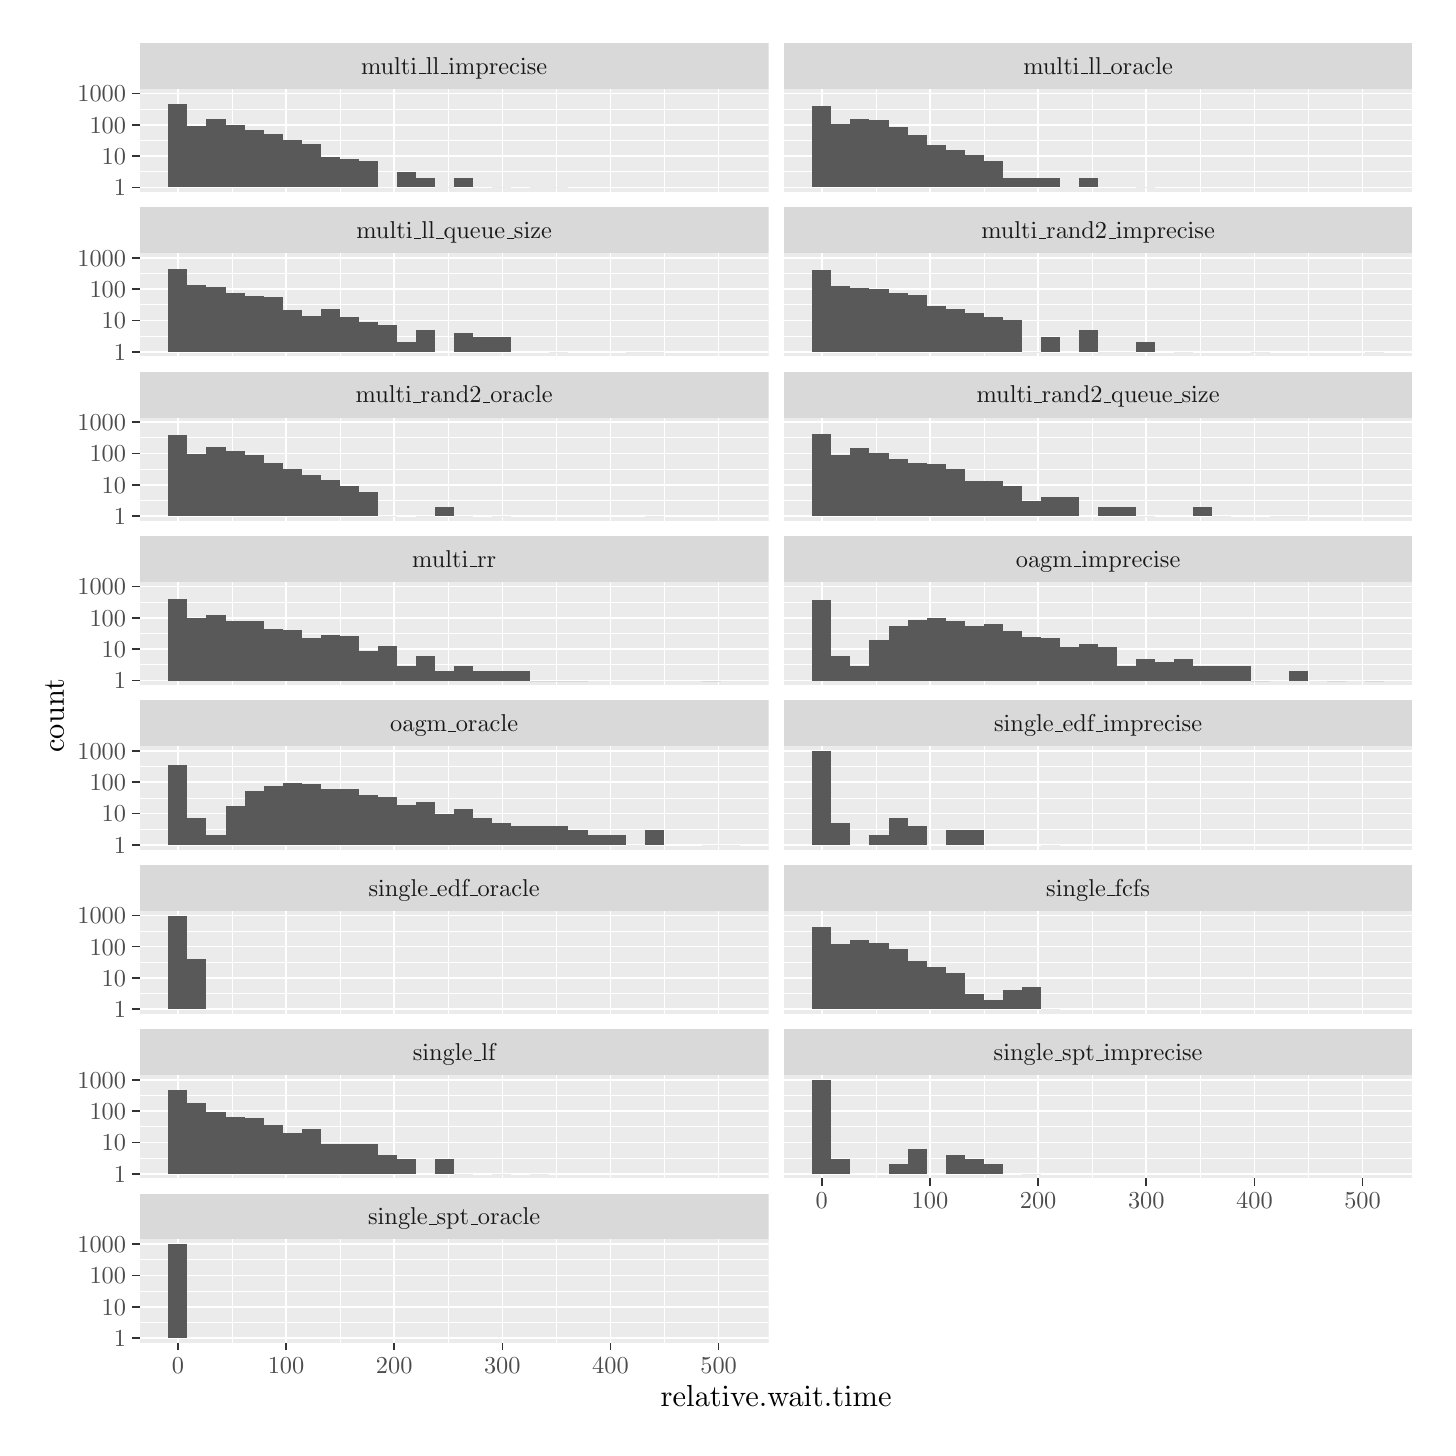
\begin{tikzpicture}[x=1pt,y=1pt]
\definecolor{fillColor}{RGB}{255,255,255}
\path[use as bounding box,fill=fillColor,fill opacity=0.00] (0,0) rectangle (505.89,505.89);
\begin{scope}
\path[clip] (  0.00,  0.00) rectangle (505.89,505.89);
\definecolor{drawColor}{RGB}{255,255,255}
\definecolor{fillColor}{RGB}{255,255,255}

\path[draw=drawColor,line width= 0.6pt,line join=round,line cap=round,fill=fillColor] (  0.00,  0.00) rectangle (505.89,505.89);
\end{scope}
\begin{scope}
\path[clip] ( 40.51,446.49) rectangle (267.70,483.82);
\definecolor{fillColor}{gray}{0.92}

\path[fill=fillColor] ( 40.51,446.49) rectangle (267.70,483.82);
\definecolor{drawColor}{RGB}{255,255,255}

\path[draw=drawColor,line width= 0.3pt,line join=round] ( 40.51,453.84) --
	(267.70,453.84);

\path[draw=drawColor,line width= 0.3pt,line join=round] ( 40.51,465.15) --
	(267.70,465.15);

\path[draw=drawColor,line width= 0.3pt,line join=round] ( 40.51,476.47) --
	(267.70,476.47);

\path[draw=drawColor,line width= 0.3pt,line join=round] ( 73.82,446.49) --
	( 73.82,483.82);

\path[draw=drawColor,line width= 0.3pt,line join=round] (112.90,446.49) --
	(112.90,483.82);

\path[draw=drawColor,line width= 0.3pt,line join=round] (151.98,446.49) --
	(151.98,483.82);

\path[draw=drawColor,line width= 0.3pt,line join=round] (191.06,446.49) --
	(191.06,483.82);

\path[draw=drawColor,line width= 0.3pt,line join=round] (230.14,446.49) --
	(230.14,483.82);

\path[draw=drawColor,line width= 0.6pt,line join=round] ( 40.51,448.19) --
	(267.70,448.19);

\path[draw=drawColor,line width= 0.6pt,line join=round] ( 40.51,459.50) --
	(267.70,459.50);

\path[draw=drawColor,line width= 0.6pt,line join=round] ( 40.51,470.81) --
	(267.70,470.81);

\path[draw=drawColor,line width= 0.6pt,line join=round] ( 40.51,482.12) --
	(267.70,482.12);

\path[draw=drawColor,line width= 0.6pt,line join=round] ( 54.28,446.49) --
	( 54.28,483.82);

\path[draw=drawColor,line width= 0.6pt,line join=round] ( 93.36,446.49) --
	( 93.36,483.82);

\path[draw=drawColor,line width= 0.6pt,line join=round] (132.44,446.49) --
	(132.44,483.82);

\path[draw=drawColor,line width= 0.6pt,line join=round] (171.52,446.49) --
	(171.52,483.82);

\path[draw=drawColor,line width= 0.6pt,line join=round] (210.60,446.49) --
	(210.60,483.82);

\path[draw=drawColor,line width= 0.6pt,line join=round] (249.68,446.49) --
	(249.68,483.82);
\definecolor{fillColor}{gray}{0.35}

\path[fill=fillColor] ( 50.84,448.19) rectangle ( 57.72,478.14);

\path[fill=fillColor] ( 57.72,448.19) rectangle ( 64.61,470.29);

\path[fill=fillColor] ( 64.61,448.19) rectangle ( 71.49,472.90);

\path[fill=fillColor] ( 71.49,448.19) rectangle ( 78.38,470.86);

\path[fill=fillColor] ( 78.38,448.19) rectangle ( 85.26,468.92);

\path[fill=fillColor] ( 85.26,448.19) rectangle ( 92.14,467.50);

\path[fill=fillColor] ( 92.14,448.19) rectangle ( 99.03,465.36);

\path[fill=fillColor] ( 99.03,448.19) rectangle (105.91,463.80);

\path[fill=fillColor] (105.91,448.19) rectangle (112.80,458.98);

\path[fill=fillColor] (112.80,448.19) rectangle (119.68,458.40);

\path[fill=fillColor] (119.68,448.19) rectangle (126.57,457.75);

\path[fill=fillColor] (133.45,448.19) rectangle (140.34,453.58);

\path[fill=fillColor] (140.34,448.19) rectangle (147.22,451.59);

\path[fill=fillColor] (147.22,448.19) rectangle (154.11,448.19);

\path[fill=fillColor] (154.11,448.19) rectangle (160.99,451.59);

\path[fill=fillColor] (167.87,448.19) rectangle (174.76,448.19);

\path[fill=fillColor] (181.64,448.19) rectangle (188.53,448.19);

\path[fill=fillColor] (188.53,448.19) rectangle (195.41,448.19);
\end{scope}
\begin{scope}
\path[clip] ( 40.51,387.09) rectangle (267.70,424.42);
\definecolor{fillColor}{gray}{0.92}

\path[fill=fillColor] ( 40.51,387.09) rectangle (267.70,424.42);
\definecolor{drawColor}{RGB}{255,255,255}

\path[draw=drawColor,line width= 0.3pt,line join=round] ( 40.51,394.44) --
	(267.70,394.44);

\path[draw=drawColor,line width= 0.3pt,line join=round] ( 40.51,405.75) --
	(267.70,405.75);

\path[draw=drawColor,line width= 0.3pt,line join=round] ( 40.51,417.07) --
	(267.70,417.07);

\path[draw=drawColor,line width= 0.3pt,line join=round] ( 73.82,387.09) --
	( 73.82,424.42);

\path[draw=drawColor,line width= 0.3pt,line join=round] (112.90,387.09) --
	(112.90,424.42);

\path[draw=drawColor,line width= 0.3pt,line join=round] (151.98,387.09) --
	(151.98,424.42);

\path[draw=drawColor,line width= 0.3pt,line join=round] (191.06,387.09) --
	(191.06,424.42);

\path[draw=drawColor,line width= 0.3pt,line join=round] (230.14,387.09) --
	(230.14,424.42);

\path[draw=drawColor,line width= 0.6pt,line join=round] ( 40.51,388.79) --
	(267.70,388.79);

\path[draw=drawColor,line width= 0.6pt,line join=round] ( 40.51,400.10) --
	(267.70,400.10);

\path[draw=drawColor,line width= 0.6pt,line join=round] ( 40.51,411.41) --
	(267.70,411.41);

\path[draw=drawColor,line width= 0.6pt,line join=round] ( 40.51,422.72) --
	(267.70,422.72);

\path[draw=drawColor,line width= 0.6pt,line join=round] ( 54.28,387.09) --
	( 54.28,424.42);

\path[draw=drawColor,line width= 0.6pt,line join=round] ( 93.36,387.09) --
	( 93.36,424.42);

\path[draw=drawColor,line width= 0.6pt,line join=round] (132.44,387.09) --
	(132.44,424.42);

\path[draw=drawColor,line width= 0.6pt,line join=round] (171.52,387.09) --
	(171.52,424.42);

\path[draw=drawColor,line width= 0.6pt,line join=round] (210.60,387.09) --
	(210.60,424.42);

\path[draw=drawColor,line width= 0.6pt,line join=round] (249.68,387.09) --
	(249.68,424.42);
\definecolor{fillColor}{gray}{0.35}

\path[fill=fillColor] ( 50.84,388.79) rectangle ( 57.72,418.85);

\path[fill=fillColor] ( 57.72,388.79) rectangle ( 64.61,412.81);

\path[fill=fillColor] ( 64.61,388.79) rectangle ( 71.49,412.18);

\path[fill=fillColor] ( 71.49,388.79) rectangle ( 78.38,409.86);

\path[fill=fillColor] ( 78.38,388.79) rectangle ( 85.26,408.82);

\path[fill=fillColor] ( 85.26,388.79) rectangle ( 92.14,408.47);

\path[fill=fillColor] ( 92.14,388.79) rectangle ( 99.03,403.97);

\path[fill=fillColor] ( 99.03,388.79) rectangle (105.91,401.75);

\path[fill=fillColor] (105.91,388.79) rectangle (112.80,404.19);

\path[fill=fillColor] (112.80,388.79) rectangle (119.68,401.39);

\path[fill=fillColor] (119.68,388.79) rectangle (126.57,399.58);

\path[fill=fillColor] (126.57,388.79) rectangle (133.45,398.35);

\path[fill=fillColor] (133.45,388.79) rectangle (140.34,392.19);

\path[fill=fillColor] (140.34,388.79) rectangle (147.22,396.69);

\path[fill=fillColor] (154.11,388.79) rectangle (160.99,395.60);

\path[fill=fillColor] (160.99,388.79) rectangle (167.87,394.18);

\path[fill=fillColor] (167.87,388.79) rectangle (174.76,394.18);

\path[fill=fillColor] (188.53,388.79) rectangle (195.41,388.79);

\path[fill=fillColor] (216.07,388.79) rectangle (222.95,388.79);

\path[fill=fillColor] (222.95,388.79) rectangle (229.84,388.79);
\end{scope}
\begin{scope}
\path[clip] ( 40.51,327.69) rectangle (267.70,365.02);
\definecolor{fillColor}{gray}{0.92}

\path[fill=fillColor] ( 40.51,327.69) rectangle (267.70,365.02);
\definecolor{drawColor}{RGB}{255,255,255}

\path[draw=drawColor,line width= 0.3pt,line join=round] ( 40.51,335.04) --
	(267.70,335.04);

\path[draw=drawColor,line width= 0.3pt,line join=round] ( 40.51,346.35) --
	(267.70,346.35);

\path[draw=drawColor,line width= 0.3pt,line join=round] ( 40.51,357.66) --
	(267.70,357.66);

\path[draw=drawColor,line width= 0.3pt,line join=round] ( 73.82,327.69) --
	( 73.82,365.02);

\path[draw=drawColor,line width= 0.3pt,line join=round] (112.90,327.69) --
	(112.90,365.02);

\path[draw=drawColor,line width= 0.3pt,line join=round] (151.98,327.69) --
	(151.98,365.02);

\path[draw=drawColor,line width= 0.3pt,line join=round] (191.06,327.69) --
	(191.06,365.02);

\path[draw=drawColor,line width= 0.3pt,line join=round] (230.14,327.69) --
	(230.14,365.02);

\path[draw=drawColor,line width= 0.6pt,line join=round] ( 40.51,329.39) --
	(267.70,329.39);

\path[draw=drawColor,line width= 0.6pt,line join=round] ( 40.51,340.70) --
	(267.70,340.70);

\path[draw=drawColor,line width= 0.6pt,line join=round] ( 40.51,352.01) --
	(267.70,352.01);

\path[draw=drawColor,line width= 0.6pt,line join=round] ( 40.51,363.32) --
	(267.70,363.32);

\path[draw=drawColor,line width= 0.6pt,line join=round] ( 54.28,327.69) --
	( 54.28,365.02);

\path[draw=drawColor,line width= 0.6pt,line join=round] ( 93.36,327.69) --
	( 93.36,365.02);

\path[draw=drawColor,line width= 0.6pt,line join=round] (132.44,327.69) --
	(132.44,365.02);

\path[draw=drawColor,line width= 0.6pt,line join=round] (171.52,327.69) --
	(171.52,365.02);

\path[draw=drawColor,line width= 0.6pt,line join=round] (210.60,327.69) --
	(210.60,365.02);

\path[draw=drawColor,line width= 0.6pt,line join=round] (249.68,327.69) --
	(249.68,365.02);
\definecolor{fillColor}{gray}{0.35}

\path[fill=fillColor] ( 50.84,329.39) rectangle ( 57.72,358.82);

\path[fill=fillColor] ( 57.72,329.39) rectangle ( 64.61,351.81);

\path[fill=fillColor] ( 64.61,329.39) rectangle ( 71.49,354.29);

\path[fill=fillColor] ( 71.49,329.39) rectangle ( 78.38,352.78);

\path[fill=fillColor] ( 78.38,329.39) rectangle ( 85.26,351.44);

\path[fill=fillColor] ( 85.26,329.39) rectangle ( 92.14,348.70);

\path[fill=fillColor] ( 92.14,329.39) rectangle ( 99.03,346.41);

\path[fill=fillColor] ( 99.03,329.39) rectangle (105.91,344.10);

\path[fill=fillColor] (105.91,329.39) rectangle (112.80,342.35);

\path[fill=fillColor] (112.80,329.39) rectangle (119.68,340.18);

\path[fill=fillColor] (119.68,329.39) rectangle (126.57,338.19);

\path[fill=fillColor] (126.57,329.39) rectangle (133.45,329.39);

\path[fill=fillColor] (140.34,329.39) rectangle (147.22,329.39);

\path[fill=fillColor] (147.22,329.39) rectangle (154.11,332.79);

\path[fill=fillColor] (154.11,329.39) rectangle (160.99,329.39);

\path[fill=fillColor] (167.87,329.39) rectangle (174.76,329.39);

\path[fill=fillColor] (222.95,329.39) rectangle (229.84,329.39);
\end{scope}
\begin{scope}
\path[clip] ( 40.51,268.29) rectangle (267.70,305.62);
\definecolor{fillColor}{gray}{0.92}

\path[fill=fillColor] ( 40.51,268.29) rectangle (267.70,305.62);
\definecolor{drawColor}{RGB}{255,255,255}

\path[draw=drawColor,line width= 0.3pt,line join=round] ( 40.51,275.64) --
	(267.70,275.64);

\path[draw=drawColor,line width= 0.3pt,line join=round] ( 40.51,286.95) --
	(267.70,286.95);

\path[draw=drawColor,line width= 0.3pt,line join=round] ( 40.51,298.26) --
	(267.70,298.26);

\path[draw=drawColor,line width= 0.3pt,line join=round] ( 73.82,268.29) --
	( 73.82,305.62);

\path[draw=drawColor,line width= 0.3pt,line join=round] (112.90,268.29) --
	(112.90,305.62);

\path[draw=drawColor,line width= 0.3pt,line join=round] (151.98,268.29) --
	(151.98,305.62);

\path[draw=drawColor,line width= 0.3pt,line join=round] (191.06,268.29) --
	(191.06,305.62);

\path[draw=drawColor,line width= 0.3pt,line join=round] (230.14,268.29) --
	(230.14,305.62);

\path[draw=drawColor,line width= 0.6pt,line join=round] ( 40.51,269.98) --
	(267.70,269.98);

\path[draw=drawColor,line width= 0.6pt,line join=round] ( 40.51,281.30) --
	(267.70,281.30);

\path[draw=drawColor,line width= 0.6pt,line join=round] ( 40.51,292.61) --
	(267.70,292.61);

\path[draw=drawColor,line width= 0.6pt,line join=round] ( 40.51,303.92) --
	(267.70,303.92);

\path[draw=drawColor,line width= 0.6pt,line join=round] ( 54.28,268.29) --
	( 54.28,305.62);

\path[draw=drawColor,line width= 0.6pt,line join=round] ( 93.36,268.29) --
	( 93.36,305.62);

\path[draw=drawColor,line width= 0.6pt,line join=round] (132.44,268.29) --
	(132.44,305.62);

\path[draw=drawColor,line width= 0.6pt,line join=round] (171.52,268.29) --
	(171.52,305.62);

\path[draw=drawColor,line width= 0.6pt,line join=round] (210.60,268.29) --
	(210.60,305.62);

\path[draw=drawColor,line width= 0.6pt,line join=round] (249.68,268.29) --
	(249.68,305.62);
\definecolor{fillColor}{gray}{0.35}

\path[fill=fillColor] ( 50.84,269.98) rectangle ( 57.72,299.56);

\path[fill=fillColor] ( 57.72,269.98) rectangle ( 64.61,292.71);

\path[fill=fillColor] ( 64.61,269.98) rectangle ( 71.49,293.63);

\path[fill=fillColor] ( 71.49,269.98) rectangle ( 78.38,291.32);

\path[fill=fillColor] ( 78.38,269.98) rectangle ( 85.26,291.39);

\path[fill=fillColor] ( 85.26,269.98) rectangle ( 92.14,288.69);

\path[fill=fillColor] ( 92.14,269.98) rectangle ( 99.03,288.11);

\path[fill=fillColor] ( 99.03,269.98) rectangle (105.91,285.17);

\path[fill=fillColor] (105.91,269.98) rectangle (112.80,286.53);

\path[fill=fillColor] (112.80,269.98) rectangle (119.68,285.99);

\path[fill=fillColor] (119.68,269.98) rectangle (126.57,280.78);

\path[fill=fillColor] (126.57,269.98) rectangle (133.45,282.59);

\path[fill=fillColor] (133.45,269.98) rectangle (140.34,275.38);

\path[fill=fillColor] (140.34,269.98) rectangle (147.22,278.79);

\path[fill=fillColor] (147.22,269.98) rectangle (154.11,273.39);

\path[fill=fillColor] (154.11,269.98) rectangle (160.99,275.38);

\path[fill=fillColor] (160.99,269.98) rectangle (167.87,273.39);

\path[fill=fillColor] (167.87,269.98) rectangle (174.76,273.39);

\path[fill=fillColor] (174.76,269.98) rectangle (181.64,273.39);

\path[fill=fillColor] (181.64,269.98) rectangle (188.53,269.98);

\path[fill=fillColor] (188.53,269.98) rectangle (195.41,269.98);

\path[fill=fillColor] (195.41,269.98) rectangle (202.30,269.98);

\path[fill=fillColor] (243.60,269.98) rectangle (250.49,269.98);
\end{scope}
\begin{scope}
\path[clip] ( 40.51,208.89) rectangle (267.70,246.22);
\definecolor{fillColor}{gray}{0.92}

\path[fill=fillColor] ( 40.51,208.89) rectangle (267.70,246.22);
\definecolor{drawColor}{RGB}{255,255,255}

\path[draw=drawColor,line width= 0.3pt,line join=round] ( 40.51,216.24) --
	(267.70,216.24);

\path[draw=drawColor,line width= 0.3pt,line join=round] ( 40.51,227.55) --
	(267.70,227.55);

\path[draw=drawColor,line width= 0.3pt,line join=round] ( 40.51,238.86) --
	(267.70,238.86);

\path[draw=drawColor,line width= 0.3pt,line join=round] ( 73.82,208.89) --
	( 73.82,246.22);

\path[draw=drawColor,line width= 0.3pt,line join=round] (112.90,208.89) --
	(112.90,246.22);

\path[draw=drawColor,line width= 0.3pt,line join=round] (151.98,208.89) --
	(151.98,246.22);

\path[draw=drawColor,line width= 0.3pt,line join=round] (191.06,208.89) --
	(191.06,246.22);

\path[draw=drawColor,line width= 0.3pt,line join=round] (230.14,208.89) --
	(230.14,246.22);

\path[draw=drawColor,line width= 0.6pt,line join=round] ( 40.51,210.58) --
	(267.70,210.58);

\path[draw=drawColor,line width= 0.6pt,line join=round] ( 40.51,221.90) --
	(267.70,221.90);

\path[draw=drawColor,line width= 0.6pt,line join=round] ( 40.51,233.21) --
	(267.70,233.21);

\path[draw=drawColor,line width= 0.6pt,line join=round] ( 40.51,244.52) --
	(267.70,244.52);

\path[draw=drawColor,line width= 0.6pt,line join=round] ( 54.28,208.89) --
	( 54.28,246.22);

\path[draw=drawColor,line width= 0.6pt,line join=round] ( 93.36,208.89) --
	( 93.36,246.22);

\path[draw=drawColor,line width= 0.6pt,line join=round] (132.44,208.89) --
	(132.44,246.22);

\path[draw=drawColor,line width= 0.6pt,line join=round] (171.52,208.89) --
	(171.52,246.22);

\path[draw=drawColor,line width= 0.6pt,line join=round] (210.60,208.89) --
	(210.60,246.22);

\path[draw=drawColor,line width= 0.6pt,line join=round] (249.68,208.89) --
	(249.68,246.22);
\definecolor{fillColor}{gray}{0.35}

\path[fill=fillColor] ( 50.84,210.58) rectangle ( 57.72,239.62);

\path[fill=fillColor] ( 57.72,210.58) rectangle ( 64.61,220.14);

\path[fill=fillColor] ( 64.61,210.58) rectangle ( 71.49,213.99);

\path[fill=fillColor] ( 71.49,210.58) rectangle ( 78.38,224.50);

\path[fill=fillColor] ( 78.38,210.58) rectangle ( 85.26,230.00);

\path[fill=fillColor] ( 85.26,210.58) rectangle ( 92.14,231.86);

\path[fill=fillColor] ( 92.14,210.58) rectangle ( 99.03,232.80);

\path[fill=fillColor] ( 99.03,210.58) rectangle (105.91,232.58);

\path[fill=fillColor] (105.91,210.58) rectangle (112.80,230.78);

\path[fill=fillColor] (112.80,210.58) rectangle (119.68,230.62);

\path[fill=fillColor] (119.68,210.58) rectangle (126.57,228.71);

\path[fill=fillColor] (126.57,210.58) rectangle (133.45,227.91);

\path[fill=fillColor] (133.45,210.58) rectangle (140.34,225.05);

\path[fill=fillColor] (140.34,210.58) rectangle (147.22,225.99);

\path[fill=fillColor] (147.22,210.58) rectangle (154.11,221.90);

\path[fill=fillColor] (154.11,210.58) rectangle (160.99,223.55);

\path[fill=fillColor] (160.99,210.58) rectangle (167.87,220.14);

\path[fill=fillColor] (167.87,210.58) rectangle (174.76,218.49);

\path[fill=fillColor] (174.76,210.58) rectangle (181.64,217.39);

\path[fill=fillColor] (181.64,210.58) rectangle (188.53,217.39);

\path[fill=fillColor] (188.53,210.58) rectangle (195.41,217.39);

\path[fill=fillColor] (195.41,210.58) rectangle (202.30,215.98);

\path[fill=fillColor] (202.30,210.58) rectangle (209.18,213.99);

\path[fill=fillColor] (209.18,210.58) rectangle (216.07,213.99);

\path[fill=fillColor] (216.07,210.58) rectangle (222.95,210.58);

\path[fill=fillColor] (222.95,210.58) rectangle (229.84,215.98);

\path[fill=fillColor] (243.60,210.58) rectangle (250.49,210.58);

\path[fill=fillColor] (250.49,210.58) rectangle (257.37,210.58);
\end{scope}
\begin{scope}
\path[clip] ( 40.51,149.49) rectangle (267.70,186.82);
\definecolor{fillColor}{gray}{0.92}

\path[fill=fillColor] ( 40.51,149.49) rectangle (267.70,186.82);
\definecolor{drawColor}{RGB}{255,255,255}

\path[draw=drawColor,line width= 0.3pt,line join=round] ( 40.51,156.84) --
	(267.70,156.84);

\path[draw=drawColor,line width= 0.3pt,line join=round] ( 40.51,168.15) --
	(267.70,168.15);

\path[draw=drawColor,line width= 0.3pt,line join=round] ( 40.51,179.46) --
	(267.70,179.46);

\path[draw=drawColor,line width= 0.3pt,line join=round] ( 73.82,149.49) --
	( 73.82,186.82);

\path[draw=drawColor,line width= 0.3pt,line join=round] (112.90,149.49) --
	(112.90,186.82);

\path[draw=drawColor,line width= 0.3pt,line join=round] (151.98,149.49) --
	(151.98,186.82);

\path[draw=drawColor,line width= 0.3pt,line join=round] (191.06,149.49) --
	(191.06,186.82);

\path[draw=drawColor,line width= 0.3pt,line join=round] (230.14,149.49) --
	(230.14,186.82);

\path[draw=drawColor,line width= 0.6pt,line join=round] ( 40.51,151.18) --
	(267.70,151.18);

\path[draw=drawColor,line width= 0.6pt,line join=round] ( 40.51,162.50) --
	(267.70,162.50);

\path[draw=drawColor,line width= 0.6pt,line join=round] ( 40.51,173.81) --
	(267.70,173.81);

\path[draw=drawColor,line width= 0.6pt,line join=round] ( 40.51,185.12) --
	(267.70,185.12);

\path[draw=drawColor,line width= 0.6pt,line join=round] ( 54.28,149.49) --
	( 54.28,186.82);

\path[draw=drawColor,line width= 0.6pt,line join=round] ( 93.36,149.49) --
	( 93.36,186.82);

\path[draw=drawColor,line width= 0.6pt,line join=round] (132.44,149.49) --
	(132.44,186.82);

\path[draw=drawColor,line width= 0.6pt,line join=round] (171.52,149.49) --
	(171.52,186.82);

\path[draw=drawColor,line width= 0.6pt,line join=round] (210.60,149.49) --
	(210.60,186.82);

\path[draw=drawColor,line width= 0.6pt,line join=round] (249.68,149.49) --
	(249.68,186.82);
\definecolor{fillColor}{gray}{0.35}

\path[fill=fillColor] ( 50.84,151.18) rectangle ( 57.72,184.92);

\path[fill=fillColor] ( 57.72,151.18) rectangle ( 64.61,169.31);
\end{scope}
\begin{scope}
\path[clip] ( 40.51, 90.09) rectangle (267.70,127.42);
\definecolor{fillColor}{gray}{0.92}

\path[fill=fillColor] ( 40.51, 90.09) rectangle (267.70,127.42);
\definecolor{drawColor}{RGB}{255,255,255}

\path[draw=drawColor,line width= 0.3pt,line join=round] ( 40.51, 97.44) --
	(267.70, 97.44);

\path[draw=drawColor,line width= 0.3pt,line join=round] ( 40.51,108.75) --
	(267.70,108.75);

\path[draw=drawColor,line width= 0.3pt,line join=round] ( 40.51,120.06) --
	(267.70,120.06);

\path[draw=drawColor,line width= 0.3pt,line join=round] ( 73.82, 90.09) --
	( 73.82,127.42);

\path[draw=drawColor,line width= 0.3pt,line join=round] (112.90, 90.09) --
	(112.90,127.42);

\path[draw=drawColor,line width= 0.3pt,line join=round] (151.98, 90.09) --
	(151.98,127.42);

\path[draw=drawColor,line width= 0.3pt,line join=round] (191.06, 90.09) --
	(191.06,127.42);

\path[draw=drawColor,line width= 0.3pt,line join=round] (230.14, 90.09) --
	(230.14,127.42);

\path[draw=drawColor,line width= 0.6pt,line join=round] ( 40.51, 91.78) --
	(267.70, 91.78);

\path[draw=drawColor,line width= 0.6pt,line join=round] ( 40.51,103.09) --
	(267.70,103.09);

\path[draw=drawColor,line width= 0.6pt,line join=round] ( 40.51,114.41) --
	(267.70,114.41);

\path[draw=drawColor,line width= 0.6pt,line join=round] ( 40.51,125.72) --
	(267.70,125.72);

\path[draw=drawColor,line width= 0.6pt,line join=round] ( 54.28, 90.09) --
	( 54.28,127.42);

\path[draw=drawColor,line width= 0.6pt,line join=round] ( 93.36, 90.09) --
	( 93.36,127.42);

\path[draw=drawColor,line width= 0.6pt,line join=round] (132.44, 90.09) --
	(132.44,127.42);

\path[draw=drawColor,line width= 0.6pt,line join=round] (171.52, 90.09) --
	(171.52,127.42);

\path[draw=drawColor,line width= 0.6pt,line join=round] (210.60, 90.09) --
	(210.60,127.42);

\path[draw=drawColor,line width= 0.6pt,line join=round] (249.68, 90.09) --
	(249.68,127.42);
\definecolor{fillColor}{gray}{0.35}

\path[fill=fillColor] ( 50.84, 91.78) rectangle ( 57.72,122.12);

\path[fill=fillColor] ( 57.72, 91.78) rectangle ( 64.61,117.16);

\path[fill=fillColor] ( 64.61, 91.78) rectangle ( 71.49,114.05);

\path[fill=fillColor] ( 71.49, 91.78) rectangle ( 78.38,112.37);

\path[fill=fillColor] ( 78.38, 91.78) rectangle ( 85.26,112.06);

\path[fill=fillColor] ( 85.26, 91.78) rectangle ( 92.14,109.52);

\path[fill=fillColor] ( 92.14, 91.78) rectangle ( 99.03,106.50);

\path[fill=fillColor] ( 99.03, 91.78) rectangle (105.91,107.79);

\path[fill=fillColor] (105.91, 91.78) rectangle (112.80,102.58);

\path[fill=fillColor] (112.80, 91.78) rectangle (119.68,102.58);

\path[fill=fillColor] (119.68, 91.78) rectangle (126.57,102.58);

\path[fill=fillColor] (126.57, 91.78) rectangle (133.45, 98.59);

\path[fill=fillColor] (133.45, 91.78) rectangle (140.34, 97.18);

\path[fill=fillColor] (147.22, 91.78) rectangle (154.11, 97.18);

\path[fill=fillColor] (154.11, 91.78) rectangle (160.99, 91.78);

\path[fill=fillColor] (167.87, 91.78) rectangle (174.76, 91.78);

\path[fill=fillColor] (181.64, 91.78) rectangle (188.53, 91.78);
\end{scope}
\begin{scope}
\path[clip] ( 40.51, 30.69) rectangle (267.70, 68.01);
\definecolor{fillColor}{gray}{0.92}

\path[fill=fillColor] ( 40.51, 30.69) rectangle (267.70, 68.01);
\definecolor{drawColor}{RGB}{255,255,255}

\path[draw=drawColor,line width= 0.3pt,line join=round] ( 40.51, 38.04) --
	(267.70, 38.04);

\path[draw=drawColor,line width= 0.3pt,line join=round] ( 40.51, 49.35) --
	(267.70, 49.35);

\path[draw=drawColor,line width= 0.3pt,line join=round] ( 40.51, 60.66) --
	(267.70, 60.66);

\path[draw=drawColor,line width= 0.3pt,line join=round] ( 73.82, 30.69) --
	( 73.82, 68.01);

\path[draw=drawColor,line width= 0.3pt,line join=round] (112.90, 30.69) --
	(112.90, 68.01);

\path[draw=drawColor,line width= 0.3pt,line join=round] (151.98, 30.69) --
	(151.98, 68.01);

\path[draw=drawColor,line width= 0.3pt,line join=round] (191.06, 30.69) --
	(191.06, 68.01);

\path[draw=drawColor,line width= 0.3pt,line join=round] (230.14, 30.69) --
	(230.14, 68.01);

\path[draw=drawColor,line width= 0.6pt,line join=round] ( 40.51, 32.38) --
	(267.70, 32.38);

\path[draw=drawColor,line width= 0.6pt,line join=round] ( 40.51, 43.69) --
	(267.70, 43.69);

\path[draw=drawColor,line width= 0.6pt,line join=round] ( 40.51, 55.01) --
	(267.70, 55.01);

\path[draw=drawColor,line width= 0.6pt,line join=round] ( 40.51, 66.32) --
	(267.70, 66.32);

\path[draw=drawColor,line width= 0.6pt,line join=round] ( 54.28, 30.69) --
	( 54.28, 68.01);

\path[draw=drawColor,line width= 0.6pt,line join=round] ( 93.36, 30.69) --
	( 93.36, 68.01);

\path[draw=drawColor,line width= 0.6pt,line join=round] (132.44, 30.69) --
	(132.44, 68.01);

\path[draw=drawColor,line width= 0.6pt,line join=round] (171.52, 30.69) --
	(171.52, 68.01);

\path[draw=drawColor,line width= 0.6pt,line join=round] (210.60, 30.69) --
	(210.60, 68.01);

\path[draw=drawColor,line width= 0.6pt,line join=round] (249.68, 30.69) --
	(249.68, 68.01);
\definecolor{fillColor}{gray}{0.35}

\path[fill=fillColor] ( 50.84, 32.38) rectangle ( 57.72, 66.32);
\end{scope}
\begin{scope}
\path[clip] (273.20,446.49) rectangle (500.39,483.82);
\definecolor{fillColor}{gray}{0.92}

\path[fill=fillColor] (273.20,446.49) rectangle (500.39,483.82);
\definecolor{drawColor}{RGB}{255,255,255}

\path[draw=drawColor,line width= 0.3pt,line join=round] (273.20,453.84) --
	(500.39,453.84);

\path[draw=drawColor,line width= 0.3pt,line join=round] (273.20,465.15) --
	(500.39,465.15);

\path[draw=drawColor,line width= 0.3pt,line join=round] (273.20,476.47) --
	(500.39,476.47);

\path[draw=drawColor,line width= 0.3pt,line join=round] (306.51,446.49) --
	(306.51,483.82);

\path[draw=drawColor,line width= 0.3pt,line join=round] (345.59,446.49) --
	(345.59,483.82);

\path[draw=drawColor,line width= 0.3pt,line join=round] (384.67,446.49) --
	(384.67,483.82);

\path[draw=drawColor,line width= 0.3pt,line join=round] (423.75,446.49) --
	(423.75,483.82);

\path[draw=drawColor,line width= 0.3pt,line join=round] (462.83,446.49) --
	(462.83,483.82);

\path[draw=drawColor,line width= 0.6pt,line join=round] (273.20,448.19) --
	(500.39,448.19);

\path[draw=drawColor,line width= 0.6pt,line join=round] (273.20,459.50) --
	(500.39,459.50);

\path[draw=drawColor,line width= 0.6pt,line join=round] (273.20,470.81) --
	(500.39,470.81);

\path[draw=drawColor,line width= 0.6pt,line join=round] (273.20,482.12) --
	(500.39,482.12);

\path[draw=drawColor,line width= 0.6pt,line join=round] (286.97,446.49) --
	(286.97,483.82);

\path[draw=drawColor,line width= 0.6pt,line join=round] (326.05,446.49) --
	(326.05,483.82);

\path[draw=drawColor,line width= 0.6pt,line join=round] (365.13,446.49) --
	(365.13,483.82);

\path[draw=drawColor,line width= 0.6pt,line join=round] (404.21,446.49) --
	(404.21,483.82);

\path[draw=drawColor,line width= 0.6pt,line join=round] (443.29,446.49) --
	(443.29,483.82);

\path[draw=drawColor,line width= 0.6pt,line join=round] (482.37,446.49) --
	(482.37,483.82);
\definecolor{fillColor}{gray}{0.35}

\path[fill=fillColor] (283.53,448.19) rectangle (290.41,477.58);

\path[fill=fillColor] (290.41,448.19) rectangle (297.30,471.19);

\path[fill=fillColor] (297.30,448.19) rectangle (304.18,472.96);

\path[fill=fillColor] (304.18,448.19) rectangle (311.07,472.53);

\path[fill=fillColor] (311.07,448.19) rectangle (317.95,470.01);

\path[fill=fillColor] (317.95,448.19) rectangle (324.83,467.00);

\path[fill=fillColor] (324.83,448.19) rectangle (331.72,463.59);

\path[fill=fillColor] (331.72,448.19) rectangle (338.60,461.81);

\path[fill=fillColor] (338.60,448.19) rectangle (345.49,459.97);

\path[fill=fillColor] (345.49,448.19) rectangle (352.37,457.75);

\path[fill=fillColor] (352.37,448.19) rectangle (359.26,451.59);

\path[fill=fillColor] (359.26,448.19) rectangle (366.14,451.59);

\path[fill=fillColor] (366.14,448.19) rectangle (373.03,451.59);

\path[fill=fillColor] (373.03,448.19) rectangle (379.91,448.19);

\path[fill=fillColor] (379.91,448.19) rectangle (386.80,451.59);

\path[fill=fillColor] (400.56,448.19) rectangle (407.45,448.19);
\end{scope}
\begin{scope}
\path[clip] (273.20,387.09) rectangle (500.39,424.42);
\definecolor{fillColor}{gray}{0.92}

\path[fill=fillColor] (273.20,387.09) rectangle (500.39,424.42);
\definecolor{drawColor}{RGB}{255,255,255}

\path[draw=drawColor,line width= 0.3pt,line join=round] (273.20,394.44) --
	(500.39,394.44);

\path[draw=drawColor,line width= 0.3pt,line join=round] (273.20,405.75) --
	(500.39,405.75);

\path[draw=drawColor,line width= 0.3pt,line join=round] (273.20,417.07) --
	(500.39,417.07);

\path[draw=drawColor,line width= 0.3pt,line join=round] (306.51,387.09) --
	(306.51,424.42);

\path[draw=drawColor,line width= 0.3pt,line join=round] (345.59,387.09) --
	(345.59,424.42);

\path[draw=drawColor,line width= 0.3pt,line join=round] (384.67,387.09) --
	(384.67,424.42);

\path[draw=drawColor,line width= 0.3pt,line join=round] (423.75,387.09) --
	(423.75,424.42);

\path[draw=drawColor,line width= 0.3pt,line join=round] (462.83,387.09) --
	(462.83,424.42);

\path[draw=drawColor,line width= 0.6pt,line join=round] (273.20,388.79) --
	(500.39,388.79);

\path[draw=drawColor,line width= 0.6pt,line join=round] (273.20,400.10) --
	(500.39,400.10);

\path[draw=drawColor,line width= 0.6pt,line join=round] (273.20,411.41) --
	(500.39,411.41);

\path[draw=drawColor,line width= 0.6pt,line join=round] (273.20,422.72) --
	(500.39,422.72);

\path[draw=drawColor,line width= 0.6pt,line join=round] (286.97,387.09) --
	(286.97,424.42);

\path[draw=drawColor,line width= 0.6pt,line join=round] (326.05,387.09) --
	(326.05,424.42);

\path[draw=drawColor,line width= 0.6pt,line join=round] (365.13,387.09) --
	(365.13,424.42);

\path[draw=drawColor,line width= 0.6pt,line join=round] (404.21,387.09) --
	(404.21,424.42);

\path[draw=drawColor,line width= 0.6pt,line join=round] (443.29,387.09) --
	(443.29,424.42);

\path[draw=drawColor,line width= 0.6pt,line join=round] (482.37,387.09) --
	(482.37,424.42);
\definecolor{fillColor}{gray}{0.35}

\path[fill=fillColor] (283.53,388.79) rectangle (290.41,418.41);

\path[fill=fillColor] (290.41,388.79) rectangle (297.30,412.54);

\path[fill=fillColor] (297.30,388.79) rectangle (304.18,411.92);

\path[fill=fillColor] (304.18,388.79) rectangle (311.07,411.51);

\path[fill=fillColor] (311.07,388.79) rectangle (317.95,409.93);

\path[fill=fillColor] (317.95,388.79) rectangle (324.83,409.14);

\path[fill=fillColor] (324.83,388.79) rectangle (331.72,405.33);

\path[fill=fillColor] (331.72,388.79) rectangle (338.60,404.19);

\path[fill=fillColor] (338.60,388.79) rectangle (345.49,402.70);

\path[fill=fillColor] (345.49,388.79) rectangle (352.37,401.39);

\path[fill=fillColor] (352.37,388.79) rectangle (359.26,400.10);

\path[fill=fillColor] (359.26,388.79) rectangle (366.14,388.79);

\path[fill=fillColor] (366.14,388.79) rectangle (373.03,394.18);

\path[fill=fillColor] (379.91,388.79) rectangle (386.80,396.69);

\path[fill=fillColor] (386.80,388.79) rectangle (393.68,388.79);

\path[fill=fillColor] (393.68,388.79) rectangle (400.56,388.79);

\path[fill=fillColor] (400.56,388.79) rectangle (407.45,392.19);

\path[fill=fillColor] (414.33,388.79) rectangle (421.22,388.79);

\path[fill=fillColor] (441.87,388.79) rectangle (448.76,388.79);

\path[fill=fillColor] (483.18,388.79) rectangle (490.06,388.79);
\end{scope}
\begin{scope}
\path[clip] (273.20,327.69) rectangle (500.39,365.02);
\definecolor{fillColor}{gray}{0.92}

\path[fill=fillColor] (273.20,327.69) rectangle (500.39,365.02);
\definecolor{drawColor}{RGB}{255,255,255}

\path[draw=drawColor,line width= 0.3pt,line join=round] (273.20,335.04) --
	(500.39,335.04);

\path[draw=drawColor,line width= 0.3pt,line join=round] (273.20,346.35) --
	(500.39,346.35);

\path[draw=drawColor,line width= 0.3pt,line join=round] (273.20,357.66) --
	(500.39,357.66);

\path[draw=drawColor,line width= 0.3pt,line join=round] (306.51,327.69) --
	(306.51,365.02);

\path[draw=drawColor,line width= 0.3pt,line join=round] (345.59,327.69) --
	(345.59,365.02);

\path[draw=drawColor,line width= 0.3pt,line join=round] (384.67,327.69) --
	(384.67,365.02);

\path[draw=drawColor,line width= 0.3pt,line join=round] (423.75,327.69) --
	(423.75,365.02);

\path[draw=drawColor,line width= 0.3pt,line join=round] (462.83,327.69) --
	(462.83,365.02);

\path[draw=drawColor,line width= 0.6pt,line join=round] (273.20,329.39) --
	(500.39,329.39);

\path[draw=drawColor,line width= 0.6pt,line join=round] (273.20,340.70) --
	(500.39,340.70);

\path[draw=drawColor,line width= 0.6pt,line join=round] (273.20,352.01) --
	(500.39,352.01);

\path[draw=drawColor,line width= 0.6pt,line join=round] (273.20,363.32) --
	(500.39,363.32);

\path[draw=drawColor,line width= 0.6pt,line join=round] (286.97,327.69) --
	(286.97,365.02);

\path[draw=drawColor,line width= 0.6pt,line join=round] (326.05,327.69) --
	(326.05,365.02);

\path[draw=drawColor,line width= 0.6pt,line join=round] (365.13,327.69) --
	(365.13,365.02);

\path[draw=drawColor,line width= 0.6pt,line join=round] (404.21,327.69) --
	(404.21,365.02);

\path[draw=drawColor,line width= 0.6pt,line join=round] (443.29,327.69) --
	(443.29,365.02);

\path[draw=drawColor,line width= 0.6pt,line join=round] (482.37,327.69) --
	(482.37,365.02);
\definecolor{fillColor}{gray}{0.35}

\path[fill=fillColor] (283.53,329.39) rectangle (290.41,358.99);

\path[fill=fillColor] (290.41,329.39) rectangle (297.30,351.38);

\path[fill=fillColor] (297.30,329.39) rectangle (304.18,353.97);

\path[fill=fillColor] (304.18,329.39) rectangle (311.07,352.11);

\path[fill=fillColor] (311.07,329.39) rectangle (317.95,349.97);

\path[fill=fillColor] (317.95,329.39) rectangle (324.83,348.40);

\path[fill=fillColor] (324.83,329.39) rectangle (331.72,348.19);

\path[fill=fillColor] (331.72,329.39) rectangle (338.60,346.26);

\path[fill=fillColor] (338.60,329.39) rectangle (345.49,341.99);

\path[fill=fillColor] (345.49,329.39) rectangle (352.37,341.99);

\path[fill=fillColor] (352.37,329.39) rectangle (359.26,340.18);

\path[fill=fillColor] (359.26,329.39) rectangle (366.14,334.78);

\path[fill=fillColor] (366.14,329.39) rectangle (373.03,336.20);

\path[fill=fillColor] (373.03,329.39) rectangle (379.91,336.20);

\path[fill=fillColor] (386.80,329.39) rectangle (393.68,332.79);

\path[fill=fillColor] (393.68,329.39) rectangle (400.56,332.79);

\path[fill=fillColor] (400.56,329.39) rectangle (407.45,329.39);

\path[fill=fillColor] (421.22,329.39) rectangle (428.10,332.79);

\path[fill=fillColor] (428.10,329.39) rectangle (434.99,329.39);

\path[fill=fillColor] (448.76,329.39) rectangle (455.64,329.39);

\path[fill=fillColor] (455.64,329.39) rectangle (462.53,329.39);
\end{scope}
\begin{scope}
\path[clip] (273.20,268.29) rectangle (500.39,305.62);
\definecolor{fillColor}{gray}{0.92}

\path[fill=fillColor] (273.20,268.29) rectangle (500.39,305.62);
\definecolor{drawColor}{RGB}{255,255,255}

\path[draw=drawColor,line width= 0.3pt,line join=round] (273.20,275.64) --
	(500.39,275.64);

\path[draw=drawColor,line width= 0.3pt,line join=round] (273.20,286.95) --
	(500.39,286.95);

\path[draw=drawColor,line width= 0.3pt,line join=round] (273.20,298.26) --
	(500.39,298.26);

\path[draw=drawColor,line width= 0.3pt,line join=round] (306.51,268.29) --
	(306.51,305.62);

\path[draw=drawColor,line width= 0.3pt,line join=round] (345.59,268.29) --
	(345.59,305.62);

\path[draw=drawColor,line width= 0.3pt,line join=round] (384.67,268.29) --
	(384.67,305.62);

\path[draw=drawColor,line width= 0.3pt,line join=round] (423.75,268.29) --
	(423.75,305.62);

\path[draw=drawColor,line width= 0.3pt,line join=round] (462.83,268.29) --
	(462.83,305.62);

\path[draw=drawColor,line width= 0.6pt,line join=round] (273.20,269.98) --
	(500.39,269.98);

\path[draw=drawColor,line width= 0.6pt,line join=round] (273.20,281.30) --
	(500.39,281.30);

\path[draw=drawColor,line width= 0.6pt,line join=round] (273.20,292.61) --
	(500.39,292.61);

\path[draw=drawColor,line width= 0.6pt,line join=round] (273.20,303.92) --
	(500.39,303.92);

\path[draw=drawColor,line width= 0.6pt,line join=round] (286.97,268.29) --
	(286.97,305.62);

\path[draw=drawColor,line width= 0.6pt,line join=round] (326.05,268.29) --
	(326.05,305.62);

\path[draw=drawColor,line width= 0.6pt,line join=round] (365.13,268.29) --
	(365.13,305.62);

\path[draw=drawColor,line width= 0.6pt,line join=round] (404.21,268.29) --
	(404.21,305.62);

\path[draw=drawColor,line width= 0.6pt,line join=round] (443.29,268.29) --
	(443.29,305.62);

\path[draw=drawColor,line width= 0.6pt,line join=round] (482.37,268.29) --
	(482.37,305.62);
\definecolor{fillColor}{gray}{0.35}

\path[fill=fillColor] (283.53,269.98) rectangle (290.41,299.21);

\path[fill=fillColor] (290.41,269.98) rectangle (297.30,278.79);

\path[fill=fillColor] (297.30,269.98) rectangle (304.18,275.38);

\path[fill=fillColor] (304.18,269.98) rectangle (311.07,284.70);

\path[fill=fillColor] (311.07,269.98) rectangle (317.95,289.85);

\path[fill=fillColor] (317.95,269.98) rectangle (324.83,291.75);

\path[fill=fillColor] (324.83,269.98) rectangle (331.72,292.41);

\path[fill=fillColor] (331.72,269.98) rectangle (338.60,291.39);

\path[fill=fillColor] (338.60,269.98) rectangle (345.49,289.58);

\path[fill=fillColor] (345.49,269.98) rectangle (352.37,290.49);

\path[fill=fillColor] (352.37,269.98) rectangle (359.26,287.72);

\path[fill=fillColor] (359.26,269.98) rectangle (366.14,285.80);

\path[fill=fillColor] (366.14,269.98) rectangle (373.03,285.17);

\path[fill=fillColor] (373.03,269.98) rectangle (379.91,282.19);

\path[fill=fillColor] (379.91,269.98) rectangle (386.80,283.29);

\path[fill=fillColor] (386.80,269.98) rectangle (393.68,282.19);

\path[fill=fillColor] (393.68,269.98) rectangle (400.56,275.38);

\path[fill=fillColor] (400.56,269.98) rectangle (407.45,277.89);

\path[fill=fillColor] (407.45,269.98) rectangle (414.33,276.80);

\path[fill=fillColor] (414.33,269.98) rectangle (421.22,277.89);

\path[fill=fillColor] (421.22,269.98) rectangle (428.10,275.38);

\path[fill=fillColor] (428.10,269.98) rectangle (434.99,275.38);

\path[fill=fillColor] (434.99,269.98) rectangle (441.87,275.38);

\path[fill=fillColor] (441.87,269.98) rectangle (448.76,269.98);

\path[fill=fillColor] (455.64,269.98) rectangle (462.53,273.39);

\path[fill=fillColor] (469.41,269.98) rectangle (476.29,269.98);

\path[fill=fillColor] (483.18,269.98) rectangle (490.06,269.98);
\end{scope}
\begin{scope}
\path[clip] (273.20,208.89) rectangle (500.39,246.22);
\definecolor{fillColor}{gray}{0.92}

\path[fill=fillColor] (273.20,208.89) rectangle (500.39,246.22);
\definecolor{drawColor}{RGB}{255,255,255}

\path[draw=drawColor,line width= 0.3pt,line join=round] (273.20,216.24) --
	(500.39,216.24);

\path[draw=drawColor,line width= 0.3pt,line join=round] (273.20,227.55) --
	(500.39,227.55);

\path[draw=drawColor,line width= 0.3pt,line join=round] (273.20,238.86) --
	(500.39,238.86);

\path[draw=drawColor,line width= 0.3pt,line join=round] (306.51,208.89) --
	(306.51,246.22);

\path[draw=drawColor,line width= 0.3pt,line join=round] (345.59,208.89) --
	(345.59,246.22);

\path[draw=drawColor,line width= 0.3pt,line join=round] (384.67,208.89) --
	(384.67,246.22);

\path[draw=drawColor,line width= 0.3pt,line join=round] (423.75,208.89) --
	(423.75,246.22);

\path[draw=drawColor,line width= 0.3pt,line join=round] (462.83,208.89) --
	(462.83,246.22);

\path[draw=drawColor,line width= 0.6pt,line join=round] (273.20,210.58) --
	(500.39,210.58);

\path[draw=drawColor,line width= 0.6pt,line join=round] (273.20,221.90) --
	(500.39,221.90);

\path[draw=drawColor,line width= 0.6pt,line join=round] (273.20,233.21) --
	(500.39,233.21);

\path[draw=drawColor,line width= 0.6pt,line join=round] (273.20,244.52) --
	(500.39,244.52);

\path[draw=drawColor,line width= 0.6pt,line join=round] (286.97,208.89) --
	(286.97,246.22);

\path[draw=drawColor,line width= 0.6pt,line join=round] (326.05,208.89) --
	(326.05,246.22);

\path[draw=drawColor,line width= 0.6pt,line join=round] (365.13,208.89) --
	(365.13,246.22);

\path[draw=drawColor,line width= 0.6pt,line join=round] (404.21,208.89) --
	(404.21,246.22);

\path[draw=drawColor,line width= 0.6pt,line join=round] (443.29,208.89) --
	(443.29,246.22);

\path[draw=drawColor,line width= 0.6pt,line join=round] (482.37,208.89) --
	(482.37,246.22);
\definecolor{fillColor}{gray}{0.35}

\path[fill=fillColor] (283.53,210.58) rectangle (290.41,244.40);

\path[fill=fillColor] (290.41,210.58) rectangle (297.30,218.49);

\path[fill=fillColor] (304.18,210.58) rectangle (311.07,213.99);

\path[fill=fillColor] (311.07,210.58) rectangle (317.95,220.14);

\path[fill=fillColor] (317.95,210.58) rectangle (324.83,217.39);

\path[fill=fillColor] (331.72,210.58) rectangle (338.60,215.98);

\path[fill=fillColor] (338.60,210.58) rectangle (345.49,215.98);

\path[fill=fillColor] (366.14,210.58) rectangle (373.03,210.58);
\end{scope}
\begin{scope}
\path[clip] (273.20,149.49) rectangle (500.39,186.82);
\definecolor{fillColor}{gray}{0.92}

\path[fill=fillColor] (273.20,149.49) rectangle (500.39,186.82);
\definecolor{drawColor}{RGB}{255,255,255}

\path[draw=drawColor,line width= 0.3pt,line join=round] (273.20,156.84) --
	(500.39,156.84);

\path[draw=drawColor,line width= 0.3pt,line join=round] (273.20,168.15) --
	(500.39,168.15);

\path[draw=drawColor,line width= 0.3pt,line join=round] (273.20,179.46) --
	(500.39,179.46);

\path[draw=drawColor,line width= 0.3pt,line join=round] (306.51,149.49) --
	(306.51,186.82);

\path[draw=drawColor,line width= 0.3pt,line join=round] (345.59,149.49) --
	(345.59,186.82);

\path[draw=drawColor,line width= 0.3pt,line join=round] (384.67,149.49) --
	(384.67,186.82);

\path[draw=drawColor,line width= 0.3pt,line join=round] (423.75,149.49) --
	(423.75,186.82);

\path[draw=drawColor,line width= 0.3pt,line join=round] (462.83,149.49) --
	(462.83,186.82);

\path[draw=drawColor,line width= 0.6pt,line join=round] (273.20,151.18) --
	(500.39,151.18);

\path[draw=drawColor,line width= 0.6pt,line join=round] (273.20,162.50) --
	(500.39,162.50);

\path[draw=drawColor,line width= 0.6pt,line join=round] (273.20,173.81) --
	(500.39,173.81);

\path[draw=drawColor,line width= 0.6pt,line join=round] (273.20,185.12) --
	(500.39,185.12);

\path[draw=drawColor,line width= 0.6pt,line join=round] (286.97,149.49) --
	(286.97,186.82);

\path[draw=drawColor,line width= 0.6pt,line join=round] (326.05,149.49) --
	(326.05,186.82);

\path[draw=drawColor,line width= 0.6pt,line join=round] (365.13,149.49) --
	(365.13,186.82);

\path[draw=drawColor,line width= 0.6pt,line join=round] (404.21,149.49) --
	(404.21,186.82);

\path[draw=drawColor,line width= 0.6pt,line join=round] (443.29,149.49) --
	(443.29,186.82);

\path[draw=drawColor,line width= 0.6pt,line join=round] (482.37,149.49) --
	(482.37,186.82);
\definecolor{fillColor}{gray}{0.35}

\path[fill=fillColor] (283.53,151.18) rectangle (290.41,180.79);

\path[fill=fillColor] (290.41,151.18) rectangle (297.30,174.74);

\path[fill=fillColor] (297.30,151.18) rectangle (304.18,176.27);

\path[fill=fillColor] (304.18,151.18) rectangle (311.07,175.13);

\path[fill=fillColor] (311.07,151.18) rectangle (317.95,172.83);

\path[fill=fillColor] (317.95,151.18) rectangle (324.83,168.79);

\path[fill=fillColor] (324.83,151.18) rectangle (331.72,166.37);

\path[fill=fillColor] (331.72,151.18) rectangle (338.60,164.15);

\path[fill=fillColor] (338.60,151.18) rectangle (345.49,156.58);

\path[fill=fillColor] (345.49,151.18) rectangle (352.37,154.59);

\path[fill=fillColor] (352.37,151.18) rectangle (359.26,157.99);

\path[fill=fillColor] (359.26,151.18) rectangle (366.14,159.09);

\path[fill=fillColor] (366.14,151.18) rectangle (373.03,151.18);
\end{scope}
\begin{scope}
\path[clip] (273.20, 90.09) rectangle (500.39,127.42);
\definecolor{fillColor}{gray}{0.92}

\path[fill=fillColor] (273.20, 90.09) rectangle (500.39,127.42);
\definecolor{drawColor}{RGB}{255,255,255}

\path[draw=drawColor,line width= 0.3pt,line join=round] (273.20, 97.44) --
	(500.39, 97.44);

\path[draw=drawColor,line width= 0.3pt,line join=round] (273.20,108.75) --
	(500.39,108.75);

\path[draw=drawColor,line width= 0.3pt,line join=round] (273.20,120.06) --
	(500.39,120.06);

\path[draw=drawColor,line width= 0.3pt,line join=round] (306.51, 90.09) --
	(306.51,127.42);

\path[draw=drawColor,line width= 0.3pt,line join=round] (345.59, 90.09) --
	(345.59,127.42);

\path[draw=drawColor,line width= 0.3pt,line join=round] (384.67, 90.09) --
	(384.67,127.42);

\path[draw=drawColor,line width= 0.3pt,line join=round] (423.75, 90.09) --
	(423.75,127.42);

\path[draw=drawColor,line width= 0.3pt,line join=round] (462.83, 90.09) --
	(462.83,127.42);

\path[draw=drawColor,line width= 0.6pt,line join=round] (273.20, 91.78) --
	(500.39, 91.78);

\path[draw=drawColor,line width= 0.6pt,line join=round] (273.20,103.09) --
	(500.39,103.09);

\path[draw=drawColor,line width= 0.6pt,line join=round] (273.20,114.41) --
	(500.39,114.41);

\path[draw=drawColor,line width= 0.6pt,line join=round] (273.20,125.72) --
	(500.39,125.72);

\path[draw=drawColor,line width= 0.6pt,line join=round] (286.97, 90.09) --
	(286.97,127.42);

\path[draw=drawColor,line width= 0.6pt,line join=round] (326.05, 90.09) --
	(326.05,127.42);

\path[draw=drawColor,line width= 0.6pt,line join=round] (365.13, 90.09) --
	(365.13,127.42);

\path[draw=drawColor,line width= 0.6pt,line join=round] (404.21, 90.09) --
	(404.21,127.42);

\path[draw=drawColor,line width= 0.6pt,line join=round] (443.29, 90.09) --
	(443.29,127.42);

\path[draw=drawColor,line width= 0.6pt,line join=round] (482.37, 90.09) --
	(482.37,127.42);
\definecolor{fillColor}{gray}{0.35}

\path[fill=fillColor] (283.53, 91.78) rectangle (290.41,125.61);

\path[fill=fillColor] (290.41, 91.78) rectangle (297.30, 97.18);

\path[fill=fillColor] (311.07, 91.78) rectangle (317.95, 95.19);

\path[fill=fillColor] (317.95, 91.78) rectangle (324.83,100.59);

\path[fill=fillColor] (331.72, 91.78) rectangle (338.60, 98.59);

\path[fill=fillColor] (338.60, 91.78) rectangle (345.49, 97.18);

\path[fill=fillColor] (345.49, 91.78) rectangle (352.37, 95.19);

\path[fill=fillColor] (359.26, 91.78) rectangle (366.14, 91.78);
\end{scope}
\begin{scope}
\path[clip] ( 40.51, 68.01) rectangle (267.70, 84.59);
\definecolor{fillColor}{gray}{0.85}

\path[fill=fillColor] ( 40.51, 68.01) rectangle (267.70, 84.59);
\definecolor{drawColor}{gray}{0.10}

\node[text=drawColor,anchor=base,inner sep=0pt, outer sep=0pt, scale=  0.88] at (154.11, 73.27) {single\_spt\_oracle};
\end{scope}
\begin{scope}
\path[clip] ( 40.51,127.42) rectangle (267.70,143.99);
\definecolor{fillColor}{gray}{0.85}

\path[fill=fillColor] ( 40.51,127.42) rectangle (267.70,143.99);
\definecolor{drawColor}{gray}{0.10}

\node[text=drawColor,anchor=base,inner sep=0pt, outer sep=0pt, scale=  0.88] at (154.11,132.67) {single\_lf};
\end{scope}
\begin{scope}
\path[clip] (273.20,127.42) rectangle (500.39,143.99);
\definecolor{fillColor}{gray}{0.85}

\path[fill=fillColor] (273.20,127.42) rectangle (500.39,143.99);
\definecolor{drawColor}{gray}{0.10}

\node[text=drawColor,anchor=base,inner sep=0pt, outer sep=0pt, scale=  0.88] at (386.80,132.67) {single\_spt\_imprecise};
\end{scope}
\begin{scope}
\path[clip] ( 40.51,186.82) rectangle (267.70,203.39);
\definecolor{fillColor}{gray}{0.85}

\path[fill=fillColor] ( 40.51,186.82) rectangle (267.70,203.39);
\definecolor{drawColor}{gray}{0.10}

\node[text=drawColor,anchor=base,inner sep=0pt, outer sep=0pt, scale=  0.88] at (154.11,192.07) {single\_edf\_oracle};
\end{scope}
\begin{scope}
\path[clip] (273.20,186.82) rectangle (500.39,203.39);
\definecolor{fillColor}{gray}{0.85}

\path[fill=fillColor] (273.20,186.82) rectangle (500.39,203.39);
\definecolor{drawColor}{gray}{0.10}

\node[text=drawColor,anchor=base,inner sep=0pt, outer sep=0pt, scale=  0.88] at (386.80,192.07) {single\_fcfs};
\end{scope}
\begin{scope}
\path[clip] ( 40.51,246.22) rectangle (267.70,262.79);
\definecolor{fillColor}{gray}{0.85}

\path[fill=fillColor] ( 40.51,246.22) rectangle (267.70,262.79);
\definecolor{drawColor}{gray}{0.10}

\node[text=drawColor,anchor=base,inner sep=0pt, outer sep=0pt, scale=  0.88] at (154.11,251.47) {oagm\_oracle};
\end{scope}
\begin{scope}
\path[clip] (273.20,246.22) rectangle (500.39,262.79);
\definecolor{fillColor}{gray}{0.85}

\path[fill=fillColor] (273.20,246.22) rectangle (500.39,262.79);
\definecolor{drawColor}{gray}{0.10}

\node[text=drawColor,anchor=base,inner sep=0pt, outer sep=0pt, scale=  0.88] at (386.80,251.47) {single\_edf\_imprecise};
\end{scope}
\begin{scope}
\path[clip] ( 40.51,305.62) rectangle (267.70,322.19);
\definecolor{fillColor}{gray}{0.85}

\path[fill=fillColor] ( 40.51,305.62) rectangle (267.70,322.19);
\definecolor{drawColor}{gray}{0.10}

\node[text=drawColor,anchor=base,inner sep=0pt, outer sep=0pt, scale=  0.88] at (154.11,310.87) {multi\_rr};
\end{scope}
\begin{scope}
\path[clip] (273.20,305.62) rectangle (500.39,322.19);
\definecolor{fillColor}{gray}{0.85}

\path[fill=fillColor] (273.20,305.62) rectangle (500.39,322.19);
\definecolor{drawColor}{gray}{0.10}

\node[text=drawColor,anchor=base,inner sep=0pt, outer sep=0pt, scale=  0.88] at (386.80,310.87) {oagm\_imprecise};
\end{scope}
\begin{scope}
\path[clip] ( 40.51,365.02) rectangle (267.70,381.59);
\definecolor{fillColor}{gray}{0.85}

\path[fill=fillColor] ( 40.51,365.02) rectangle (267.70,381.59);
\definecolor{drawColor}{gray}{0.10}

\node[text=drawColor,anchor=base,inner sep=0pt, outer sep=0pt, scale=  0.88] at (154.11,370.27) {multi\_rand2\_oracle};
\end{scope}
\begin{scope}
\path[clip] (273.20,365.02) rectangle (500.39,381.59);
\definecolor{fillColor}{gray}{0.85}

\path[fill=fillColor] (273.20,365.02) rectangle (500.39,381.59);
\definecolor{drawColor}{gray}{0.10}

\node[text=drawColor,anchor=base,inner sep=0pt, outer sep=0pt, scale=  0.88] at (386.80,370.27) {multi\_rand2\_queue\_size};
\end{scope}
\begin{scope}
\path[clip] ( 40.51,424.42) rectangle (267.70,440.99);
\definecolor{fillColor}{gray}{0.85}

\path[fill=fillColor] ( 40.51,424.42) rectangle (267.70,440.99);
\definecolor{drawColor}{gray}{0.10}

\node[text=drawColor,anchor=base,inner sep=0pt, outer sep=0pt, scale=  0.88] at (154.11,429.67) {multi\_ll\_queue\_size};
\end{scope}
\begin{scope}
\path[clip] (273.20,424.42) rectangle (500.39,440.99);
\definecolor{fillColor}{gray}{0.85}

\path[fill=fillColor] (273.20,424.42) rectangle (500.39,440.99);
\definecolor{drawColor}{gray}{0.10}

\node[text=drawColor,anchor=base,inner sep=0pt, outer sep=0pt, scale=  0.88] at (386.80,429.67) {multi\_rand2\_imprecise};
\end{scope}
\begin{scope}
\path[clip] ( 40.51,483.82) rectangle (267.70,500.39);
\definecolor{fillColor}{gray}{0.85}

\path[fill=fillColor] ( 40.51,483.82) rectangle (267.70,500.39);
\definecolor{drawColor}{gray}{0.10}

\node[text=drawColor,anchor=base,inner sep=0pt, outer sep=0pt, scale=  0.88] at (154.11,489.07) {multi\_ll\_imprecise};
\end{scope}
\begin{scope}
\path[clip] (273.20,483.82) rectangle (500.39,500.39);
\definecolor{fillColor}{gray}{0.85}

\path[fill=fillColor] (273.20,483.82) rectangle (500.39,500.39);
\definecolor{drawColor}{gray}{0.10}

\node[text=drawColor,anchor=base,inner sep=0pt, outer sep=0pt, scale=  0.88] at (386.80,489.07) {multi\_ll\_oracle};
\end{scope}
\begin{scope}
\path[clip] (  0.00,  0.00) rectangle (505.89,505.89);
\definecolor{drawColor}{gray}{0.20}

\path[draw=drawColor,line width= 0.6pt,line join=round] ( 54.28, 27.94) --
	( 54.28, 30.69);

\path[draw=drawColor,line width= 0.6pt,line join=round] ( 93.36, 27.94) --
	( 93.36, 30.69);

\path[draw=drawColor,line width= 0.6pt,line join=round] (132.44, 27.94) --
	(132.44, 30.69);

\path[draw=drawColor,line width= 0.6pt,line join=round] (171.52, 27.94) --
	(171.52, 30.69);

\path[draw=drawColor,line width= 0.6pt,line join=round] (210.60, 27.94) --
	(210.60, 30.69);

\path[draw=drawColor,line width= 0.6pt,line join=round] (249.68, 27.94) --
	(249.68, 30.69);
\end{scope}
\begin{scope}
\path[clip] (  0.00,  0.00) rectangle (505.89,505.89);
\definecolor{drawColor}{gray}{0.30}

\node[text=drawColor,anchor=base,inner sep=0pt, outer sep=0pt, scale=  0.88] at ( 54.28, 19.68) {0};

\node[text=drawColor,anchor=base,inner sep=0pt, outer sep=0pt, scale=  0.88] at ( 93.36, 19.68) {100};

\node[text=drawColor,anchor=base,inner sep=0pt, outer sep=0pt, scale=  0.88] at (132.44, 19.68) {200};

\node[text=drawColor,anchor=base,inner sep=0pt, outer sep=0pt, scale=  0.88] at (171.52, 19.68) {300};

\node[text=drawColor,anchor=base,inner sep=0pt, outer sep=0pt, scale=  0.88] at (210.60, 19.68) {400};

\node[text=drawColor,anchor=base,inner sep=0pt, outer sep=0pt, scale=  0.88] at (249.68, 19.68) {500};
\end{scope}
\begin{scope}
\path[clip] (  0.00,  0.00) rectangle (505.89,505.89);
\definecolor{drawColor}{gray}{0.20}

\path[draw=drawColor,line width= 0.6pt,line join=round] (286.97, 87.34) --
	(286.97, 90.09);

\path[draw=drawColor,line width= 0.6pt,line join=round] (326.05, 87.34) --
	(326.05, 90.09);

\path[draw=drawColor,line width= 0.6pt,line join=round] (365.13, 87.34) --
	(365.13, 90.09);

\path[draw=drawColor,line width= 0.6pt,line join=round] (404.21, 87.34) --
	(404.21, 90.09);

\path[draw=drawColor,line width= 0.6pt,line join=round] (443.29, 87.34) --
	(443.29, 90.09);

\path[draw=drawColor,line width= 0.6pt,line join=round] (482.37, 87.34) --
	(482.37, 90.09);
\end{scope}
\begin{scope}
\path[clip] (  0.00,  0.00) rectangle (505.89,505.89);
\definecolor{drawColor}{gray}{0.30}

\node[text=drawColor,anchor=base,inner sep=0pt, outer sep=0pt, scale=  0.88] at (286.97, 79.08) {0};

\node[text=drawColor,anchor=base,inner sep=0pt, outer sep=0pt, scale=  0.88] at (326.05, 79.08) {100};

\node[text=drawColor,anchor=base,inner sep=0pt, outer sep=0pt, scale=  0.88] at (365.13, 79.08) {200};

\node[text=drawColor,anchor=base,inner sep=0pt, outer sep=0pt, scale=  0.88] at (404.21, 79.08) {300};

\node[text=drawColor,anchor=base,inner sep=0pt, outer sep=0pt, scale=  0.88] at (443.29, 79.08) {400};

\node[text=drawColor,anchor=base,inner sep=0pt, outer sep=0pt, scale=  0.88] at (482.37, 79.08) {500};
\end{scope}
\begin{scope}
\path[clip] (  0.00,  0.00) rectangle (505.89,505.89);
\definecolor{drawColor}{gray}{0.30}

\node[text=drawColor,anchor=base east,inner sep=0pt, outer sep=0pt, scale=  0.88] at ( 35.56,445.16) {1};

\node[text=drawColor,anchor=base east,inner sep=0pt, outer sep=0pt, scale=  0.88] at ( 35.56,456.47) {10};

\node[text=drawColor,anchor=base east,inner sep=0pt, outer sep=0pt, scale=  0.88] at ( 35.56,467.78) {100};

\node[text=drawColor,anchor=base east,inner sep=0pt, outer sep=0pt, scale=  0.88] at ( 35.56,479.09) {1000};
\end{scope}
\begin{scope}
\path[clip] (  0.00,  0.00) rectangle (505.89,505.89);
\definecolor{drawColor}{gray}{0.20}

\path[draw=drawColor,line width= 0.6pt,line join=round] ( 37.76,448.19) --
	( 40.51,448.19);

\path[draw=drawColor,line width= 0.6pt,line join=round] ( 37.76,459.50) --
	( 40.51,459.50);

\path[draw=drawColor,line width= 0.6pt,line join=round] ( 37.76,470.81) --
	( 40.51,470.81);

\path[draw=drawColor,line width= 0.6pt,line join=round] ( 37.76,482.12) --
	( 40.51,482.12);
\end{scope}
\begin{scope}
\path[clip] (  0.00,  0.00) rectangle (505.89,505.89);
\definecolor{drawColor}{gray}{0.30}

\node[text=drawColor,anchor=base east,inner sep=0pt, outer sep=0pt, scale=  0.88] at ( 35.56,385.76) {1};

\node[text=drawColor,anchor=base east,inner sep=0pt, outer sep=0pt, scale=  0.88] at ( 35.56,397.07) {10};

\node[text=drawColor,anchor=base east,inner sep=0pt, outer sep=0pt, scale=  0.88] at ( 35.56,408.38) {100};

\node[text=drawColor,anchor=base east,inner sep=0pt, outer sep=0pt, scale=  0.88] at ( 35.56,419.69) {1000};
\end{scope}
\begin{scope}
\path[clip] (  0.00,  0.00) rectangle (505.89,505.89);
\definecolor{drawColor}{gray}{0.20}

\path[draw=drawColor,line width= 0.6pt,line join=round] ( 37.76,388.79) --
	( 40.51,388.79);

\path[draw=drawColor,line width= 0.6pt,line join=round] ( 37.76,400.10) --
	( 40.51,400.10);

\path[draw=drawColor,line width= 0.6pt,line join=round] ( 37.76,411.41) --
	( 40.51,411.41);

\path[draw=drawColor,line width= 0.6pt,line join=round] ( 37.76,422.72) --
	( 40.51,422.72);
\end{scope}
\begin{scope}
\path[clip] (  0.00,  0.00) rectangle (505.89,505.89);
\definecolor{drawColor}{gray}{0.30}

\node[text=drawColor,anchor=base east,inner sep=0pt, outer sep=0pt, scale=  0.88] at ( 35.56,326.35) {1};

\node[text=drawColor,anchor=base east,inner sep=0pt, outer sep=0pt, scale=  0.88] at ( 35.56,337.67) {10};

\node[text=drawColor,anchor=base east,inner sep=0pt, outer sep=0pt, scale=  0.88] at ( 35.56,348.98) {100};

\node[text=drawColor,anchor=base east,inner sep=0pt, outer sep=0pt, scale=  0.88] at ( 35.56,360.29) {1000};
\end{scope}
\begin{scope}
\path[clip] (  0.00,  0.00) rectangle (505.89,505.89);
\definecolor{drawColor}{gray}{0.20}

\path[draw=drawColor,line width= 0.6pt,line join=round] ( 37.76,329.39) --
	( 40.51,329.39);

\path[draw=drawColor,line width= 0.6pt,line join=round] ( 37.76,340.70) --
	( 40.51,340.70);

\path[draw=drawColor,line width= 0.6pt,line join=round] ( 37.76,352.01) --
	( 40.51,352.01);

\path[draw=drawColor,line width= 0.6pt,line join=round] ( 37.76,363.32) --
	( 40.51,363.32);
\end{scope}
\begin{scope}
\path[clip] (  0.00,  0.00) rectangle (505.89,505.89);
\definecolor{drawColor}{gray}{0.30}

\node[text=drawColor,anchor=base east,inner sep=0pt, outer sep=0pt, scale=  0.88] at ( 35.56,266.95) {1};

\node[text=drawColor,anchor=base east,inner sep=0pt, outer sep=0pt, scale=  0.88] at ( 35.56,278.27) {10};

\node[text=drawColor,anchor=base east,inner sep=0pt, outer sep=0pt, scale=  0.88] at ( 35.56,289.58) {100};

\node[text=drawColor,anchor=base east,inner sep=0pt, outer sep=0pt, scale=  0.88] at ( 35.56,300.89) {1000};
\end{scope}
\begin{scope}
\path[clip] (  0.00,  0.00) rectangle (505.89,505.89);
\definecolor{drawColor}{gray}{0.20}

\path[draw=drawColor,line width= 0.6pt,line join=round] ( 37.76,269.98) --
	( 40.51,269.98);

\path[draw=drawColor,line width= 0.6pt,line join=round] ( 37.76,281.30) --
	( 40.51,281.30);

\path[draw=drawColor,line width= 0.6pt,line join=round] ( 37.76,292.61) --
	( 40.51,292.61);

\path[draw=drawColor,line width= 0.6pt,line join=round] ( 37.76,303.92) --
	( 40.51,303.92);
\end{scope}
\begin{scope}
\path[clip] (  0.00,  0.00) rectangle (505.89,505.89);
\definecolor{drawColor}{gray}{0.30}

\node[text=drawColor,anchor=base east,inner sep=0pt, outer sep=0pt, scale=  0.88] at ( 35.56,207.55) {1};

\node[text=drawColor,anchor=base east,inner sep=0pt, outer sep=0pt, scale=  0.88] at ( 35.56,218.87) {10};

\node[text=drawColor,anchor=base east,inner sep=0pt, outer sep=0pt, scale=  0.88] at ( 35.56,230.18) {100};

\node[text=drawColor,anchor=base east,inner sep=0pt, outer sep=0pt, scale=  0.88] at ( 35.56,241.49) {1000};
\end{scope}
\begin{scope}
\path[clip] (  0.00,  0.00) rectangle (505.89,505.89);
\definecolor{drawColor}{gray}{0.20}

\path[draw=drawColor,line width= 0.6pt,line join=round] ( 37.76,210.58) --
	( 40.51,210.58);

\path[draw=drawColor,line width= 0.6pt,line join=round] ( 37.76,221.90) --
	( 40.51,221.90);

\path[draw=drawColor,line width= 0.6pt,line join=round] ( 37.76,233.21) --
	( 40.51,233.21);

\path[draw=drawColor,line width= 0.6pt,line join=round] ( 37.76,244.52) --
	( 40.51,244.52);
\end{scope}
\begin{scope}
\path[clip] (  0.00,  0.00) rectangle (505.89,505.89);
\definecolor{drawColor}{gray}{0.30}

\node[text=drawColor,anchor=base east,inner sep=0pt, outer sep=0pt, scale=  0.88] at ( 35.56,148.15) {1};

\node[text=drawColor,anchor=base east,inner sep=0pt, outer sep=0pt, scale=  0.88] at ( 35.56,159.47) {10};

\node[text=drawColor,anchor=base east,inner sep=0pt, outer sep=0pt, scale=  0.88] at ( 35.56,170.78) {100};

\node[text=drawColor,anchor=base east,inner sep=0pt, outer sep=0pt, scale=  0.88] at ( 35.56,182.09) {1000};
\end{scope}
\begin{scope}
\path[clip] (  0.00,  0.00) rectangle (505.89,505.89);
\definecolor{drawColor}{gray}{0.20}

\path[draw=drawColor,line width= 0.6pt,line join=round] ( 37.76,151.18) --
	( 40.51,151.18);

\path[draw=drawColor,line width= 0.6pt,line join=round] ( 37.76,162.50) --
	( 40.51,162.50);

\path[draw=drawColor,line width= 0.6pt,line join=round] ( 37.76,173.81) --
	( 40.51,173.81);

\path[draw=drawColor,line width= 0.6pt,line join=round] ( 37.76,185.12) --
	( 40.51,185.12);
\end{scope}
\begin{scope}
\path[clip] (  0.00,  0.00) rectangle (505.89,505.89);
\definecolor{drawColor}{gray}{0.30}

\node[text=drawColor,anchor=base east,inner sep=0pt, outer sep=0pt, scale=  0.88] at ( 35.56, 88.75) {1};

\node[text=drawColor,anchor=base east,inner sep=0pt, outer sep=0pt, scale=  0.88] at ( 35.56,100.06) {10};

\node[text=drawColor,anchor=base east,inner sep=0pt, outer sep=0pt, scale=  0.88] at ( 35.56,111.38) {100};

\node[text=drawColor,anchor=base east,inner sep=0pt, outer sep=0pt, scale=  0.88] at ( 35.56,122.69) {1000};
\end{scope}
\begin{scope}
\path[clip] (  0.00,  0.00) rectangle (505.89,505.89);
\definecolor{drawColor}{gray}{0.20}

\path[draw=drawColor,line width= 0.6pt,line join=round] ( 37.76, 91.78) --
	( 40.51, 91.78);

\path[draw=drawColor,line width= 0.6pt,line join=round] ( 37.76,103.09) --
	( 40.51,103.09);

\path[draw=drawColor,line width= 0.6pt,line join=round] ( 37.76,114.41) --
	( 40.51,114.41);

\path[draw=drawColor,line width= 0.6pt,line join=round] ( 37.76,125.72) --
	( 40.51,125.72);
\end{scope}
\begin{scope}
\path[clip] (  0.00,  0.00) rectangle (505.89,505.89);
\definecolor{drawColor}{gray}{0.30}

\node[text=drawColor,anchor=base east,inner sep=0pt, outer sep=0pt, scale=  0.88] at ( 35.56, 29.35) {1};

\node[text=drawColor,anchor=base east,inner sep=0pt, outer sep=0pt, scale=  0.88] at ( 35.56, 40.66) {10};

\node[text=drawColor,anchor=base east,inner sep=0pt, outer sep=0pt, scale=  0.88] at ( 35.56, 51.98) {100};

\node[text=drawColor,anchor=base east,inner sep=0pt, outer sep=0pt, scale=  0.88] at ( 35.56, 63.29) {1000};
\end{scope}
\begin{scope}
\path[clip] (  0.00,  0.00) rectangle (505.89,505.89);
\definecolor{drawColor}{gray}{0.20}

\path[draw=drawColor,line width= 0.6pt,line join=round] ( 37.76, 32.38) --
	( 40.51, 32.38);

\path[draw=drawColor,line width= 0.6pt,line join=round] ( 37.76, 43.69) --
	( 40.51, 43.69);

\path[draw=drawColor,line width= 0.6pt,line join=round] ( 37.76, 55.01) --
	( 40.51, 55.01);

\path[draw=drawColor,line width= 0.6pt,line join=round] ( 37.76, 66.32) --
	( 40.51, 66.32);
\end{scope}
\begin{scope}
\path[clip] (  0.00,  0.00) rectangle (505.89,505.89);
\definecolor{drawColor}{RGB}{0,0,0}

\node[text=drawColor,anchor=base,inner sep=0pt, outer sep=0pt, scale=  1.10] at (270.45,  7.64) {relative.wait.time};
\end{scope}
\begin{scope}
\path[clip] (  0.00,  0.00) rectangle (505.89,505.89);
\definecolor{drawColor}{RGB}{0,0,0}

\node[text=drawColor,rotate= 90.00,anchor=base,inner sep=0pt, outer sep=0pt, scale=  1.10] at ( 13.08,257.25) {count};
\end{scope}
\end{tikzpicture}
